\chapter{General Discussion}\thumbforchapter
\newpage

\section{The scientific dogma of the phylotypic stage}

\begin{shadequote}[c]{George Box}
All models are wrong, but some are useful.
\end{shadequote}

While historically the phylotypic stage has predominantly been examined and described through qualitative methods, the 21\textsuperscript{st} century started a paradigm shift towards a more quantitative and data-driven approach to understanding this phenomenon\cite{Chan2021}. The first notable quantitative investigation into the phylotypic stage was done by Bininda-Emonds \textit{et al.}, where they calculated temporal conservation as the order in which morphological embryonic features appear in vertebrates\cite{OlafRP2003}. However, it wasn't until the early 2010s that the field truly embraced quantitative methodologies with the simultaneous publication of two groundbreaking studies in Nature\cite{Kalinka2010, DomazetLoso2010}. In these works, Domazet-Lošo \textit{et al.} investigated the average developmental age of transcripts in \textit{D. rerio} and \textit{D. melanogaster}, whilst at the same time, Kalinka \textit{et al.} explored the temporal transcriptome similarities across different \textit{Drosophila} species. These molecular studies opened a new line of research to the quantitative basis of the phylotypic stage. The quantitative support for the phylotypic stage appeared stronger and stronger with each new study. So strong, that we quickly forgot all the nonconforming studies.

The Transcriptome Age Index (TAI), as introduced by Domazet-Lošo \textit{et al.}, is a metric of the average evolutionary age of transcripts over time\cite{DomazetLoso2010}. Evolutionary age is determined as the number of taxonomic branches to which a gene can be traced back. The central idea of the TAI is that temporal changes in gene expression provide insights into the degree of conservation during development. However, a re-analysis conducted by Piasecka \textit{et al.} raised some critical points about the methodology\cite{Piasecka2013}. Their investigation revealed that the TAI is heavily influenced by a relatively small subset of genes due to major differences in transcript levels per gene (transcriptomic data is notoriously heteroscedastic). Log transforming the data, which is a standard processing step for this type of data, completely invalidates the results of the original study. One might expect such a dependency on data transformation to cast doubts on the reliability of a/the method. Surprisingly, the opposite appears to be true. The original study introducing the TAI has been cited 88 times between 2010 and 2013, and has been cited 359 times since Piasecka \textit{et al.}'s publication (covering the years 2014-2023). As it turns out, you can now analyze the data with and without transformation, and keep the results that reinforce your preferred hypothesis. A notable example of this is found in Wu \textit{et al.}'s study on Spiralian development\cite{Wu2019}. In their analysis of untransformed data for \textit{Crassostrea gigas}, \textit{Haliotis discus hannai}, and \textit{Perinereis aibuhitensis}, they claim to have found an inverse hourglass pattern. However, their supplementary data reveals a different pattern for \textit{Crassostrea gigas} after square root transformation, shifting from an inverse hourglass to a funnel shape. Remarkably, this crucial finding receives minimal attention in the study, with the authors merely stating that at least the transformed data does not show an hourglass-like pattern. Moreover, the transformed TAI of the other two species are not even shown. It is also noteworthy that the inverse hourglass pattern of \textit{Perinereis aibuhitensis} of untransformed data can be attributed to random noise. Where this study should be taken with a grain of salt, it has sparked an exchange among three influential evolutionary-developmental biologists - Pavel Tomanczak, Denis Duboule, and Andreas Hejnol - on Twitter (now X), about the universality of the hourglass model\cite{hejnoltwitter}. It is worth mentioning that Andreas Hejnol has authored two critical reviews of previous studies that asserted the universality of the phylotypic stage\cite{Dunn2018,hejnol2016}.

The work of Barbara Piasecka, where she showed that the pattern of the TAI is caused by a subset of all genes was led by Marc Robinson-Rechavi. The main work of this study was not about the TAI, but about using a multitude of different metrics to estimate temporal evolutionary conservation. Their conclusion is that different metrics give different results. In his personal blog, Marc Robinson-Rechavi concludes \say{First, that biology is complicated, and insisting on answers such as « the hourglass exists (and explains diverse data) » or « it doesn’t » may not be the best strategy. Second, that the technical details are very important}\cite{robinsonrechaviblog}. Marc Robinson-Rechavi's later career, however, appears to have diverged from his earlier conclusions. He has made assertive claims concerning the ortholog conjecture\cite{KryuchkovaMostacci2016} and the hourglass model of conservation\cite{Liu2020,Liu2021,marletaz2018}. A re-analysis by Casey Dunn \textit{et al.} identified methodological issues with their analysis of the ortholog conjecture\cite{Dunn2018}, and in chapter \textbf{X} I discuss in detail the methodological problems of two of his studies related to the hourglass model.

In 2003, Bininda-Emonds \textit{et al.} conducted a quantitative study of the phylotypic stage, which was revisited by Gerardo A. Cordero \textit{et al.} seventeen years later\cite{OlafRP2003, Cordero2020}. Both studies were about the quantitative temporal analysis of morphological characteristics. To the best of my knowledge, these are the only quantitative analyses of morphological characteristics with respect to the phylotypic stage. The initial findings of Bininda-Emonds et al. revealed an unexpected inverse hourglass pattern in morphological rankings, a discovery that challenged existing assumptions. However, the later study of Cordero \textit{et al.} shows precisely the opposite - an hourglass pattern. Surprisingly, Cordero \textit{et al.} only comment that the difference between these two studies \textit{could} be caused by a difference in morphological characteristics, methodology, and species used, without any further analysis of the differences. The main analysis of Bininda-Emonds \textit{et al.} is a mean-variance plot, something that takes 5 minutes to generate, and it is truly puzzling why Cordero \textit{et al.} did not repeat this analysis. \textit{change into sth like, they were close as indeed the difference could be fully explained by a difference in methodology}

In 2016, Levin \textit{et al.} introduced the transcriptomic inverse hourglass model as a potential method for distinguishing between different phyla\cite{Levin2016}. However, this study has been rightfully criticized by Casey Dunn and Andreas Hejnol for its lack of a within-phylum control\cite{hejnol2016} and incorrect statistical methods\cite{Dunn2018}. Given the ambitious claim of a "universal" phylotypic stage characterized by high similarity within phyla but low similarity between phyla, it is somewhat perplexing that these criticisms have not yet been addressed by Levin \textit{et al}. What makes the situation even more perplexing is that another group of evolutionary developmental biologists compared the embryonic development of deuterostomes and the chordate amphioxus - a between-phyla comparison. Astonishingly, they uncovered an hourglass-like pattern\cite{PerezPosada2022}, directly contradicting Levin \textit{et al.}'s inverse hourglass model, but fail to comment on this. In Chapter XXX, I present evidence that the transcriptomic inverse hourglass is a statistical artifact resulting from normalization rather than an accurate representation of temporal conservation. 

Yoav Mayshar \textit{et al.} studied the phylotypic stage and the hourglass model from a single-cell point of view\cite{Mayshar2023}. Their research involved a comparative analysis of cell type proportions during the development of rabbit and mouse embryos. However, in Chapter X, I show that both the rabbit time series and the mouse time series exhibit discontinuous patterns. These discontinuities significantly influence the temporal correlations between the two species. This discontinuous pattern in cell-type proportions could be interpreted as indicative of a mid-developmental transition, resembling an inverse hourglass-like pattern. What raises questions is Mayshar \textit{et al.}'s interpretation of this data. They perceive the pattern as confirming the traditional hourglass model. This leads to the question of why such a fundamental problem of their analysis was not detected during the peer review process, especially considering that the study was published in Cell, one of the most prestigious scientific journals. When I asked Y. Mayshar on Twitter if their results perhaps represent an inverse hourglass, he commented with \say{this basically shows convergence of frequencies of cell states at \textasciitilde e7.5-e8, preceding what would be normally considered as the phylotypic stage, though this is pretty vaguely defined...}. 
\textit{I can also mention the paper was on biorxiv for a while and no one responded}

\begin{figure}
    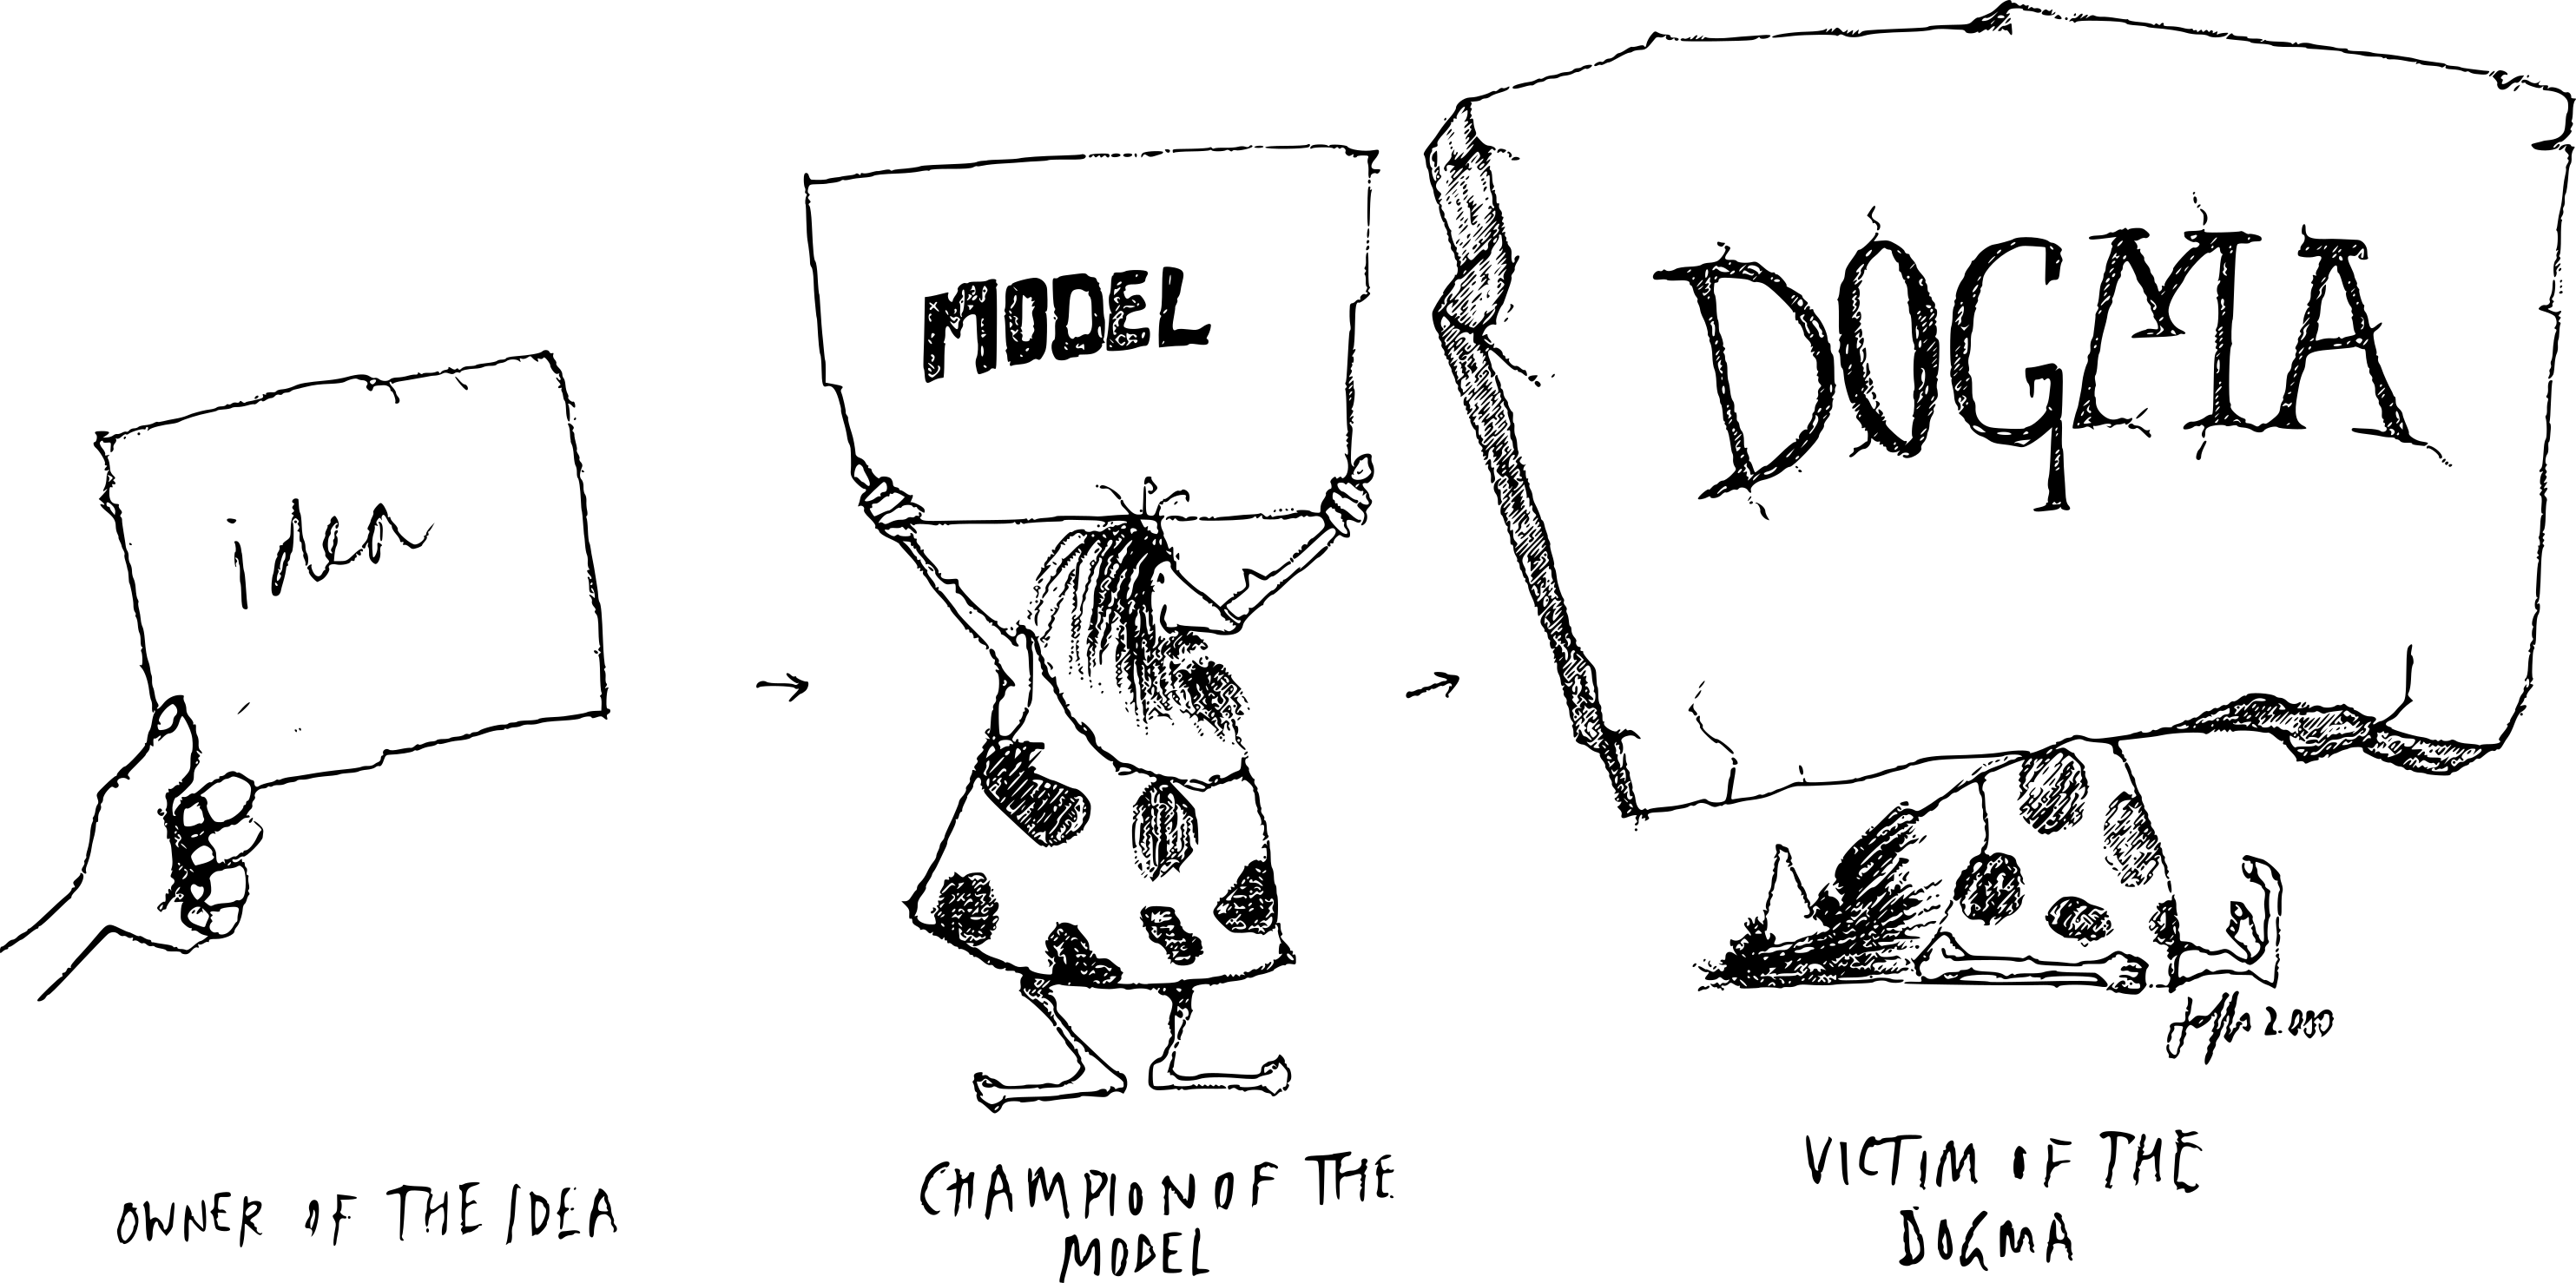
\includegraphics[width=\linewidth]{ch.discussion/imgs/dogma.png}
    \caption{\textbf{The phylotypic stage as a (crushing) scientific dogma?} \cite{Caveman2000}.}
    \label{fig:dogma}
\end{figure}

There appears to be a concerning lack of genuine effort to understand or engage with one another's work within the field. Many studies, it seems, are riddled with glaring methodological issues that often go unaddressed, as long as they align with our prior beliefs. In chapters X AND Y I show and discuss a series of newly discovered problems with comparative approaches. I fear that highlighting these problems won't actually matter, as people will continue to believe their pet theories, and there will always be some methodology that in a way affirms it. For instance, during the early stages of my PhD, I had a meeting with one of the co-authors of the papers that applies transcriptomic comparisons between \textit{D. rerio} and \textit{X. tropicalis}\cite{marletaz2018}. He is a staunch believer of the hourglass model, and even has a tattoo of it! I shared some of my preliminary findings with him, which pointed to the inverse hourglass being an artifact of normalization. I also expressed my concerns regarding the methodology employed in their analysis. Surprisingly, he brushed off my concerns, stating that he was not directly involved in that particular analysis and thus saw no need to discuss its potential issues. Similarly, a colleague in my department once commented that despite my work showing that virtually all quantitative methodologies used in our field are flawed, the undeniable fact remains that the phylotypic stage does, in fact, exist.

Based on my own re-analyses, it appears most methodologies actually can not reject the null model. The null model for evolutionary embryonic development would be that there is no specific stage of higher or lower temporal conservation. To summarize my main findings:
\begin{itemize}
    \item The hourglass-like pattern between zebrafish and frogs based on transcriptomic correlations can be explained by within-species correlations alone.
    \item The pattern of cell type proportion similarity between rabbits and mice, which is wrongfully called an hourglass, can be explained by discontinuous temporal sampling.
    \item Both the transcriptomic between-phyla inverse hourglass pattern and the morphological within-phylum inverse hourglass pattern are fully reproduced by simulated data with no specific temporal conservation.
    \item Only the \textit{Drosophila} enhancer conservation re-analysis results in a stage of maximum similarity, albeit at a different point than found by the original authors. Moreover, I simply do not agree with the methodological approach of this analysis.
\end{itemize}
\noindent
Altogether, I have found little evidence to reject the null hypothesis of constant temporal conservation based on quantitative data.

Furthermore, there is no consensus on what is actually expected to be conserved. The original observation that vertebrate embryos, perhaps, look more like each other at certain points in development than at other times, says nothing about the molecular basis for this. It has been quantitatively studied on the basis of embryonic lethality\cite{Uchida2018}, morphology\cite{OlafRP2003,Cordero2020}, DNA sequence conservation\cite{Piasecka2013,Quint2012,Liu2021} and activation order\cite{Uesaka2019}, cell type proportion\cite{Mayshar2023}, and whole-transcriptome similarity\cite{Piasecka2013,Irie2011,marletaz2018,Liu2020,Leong2021,PerezPosada2022,Kalinka2010}, with differing results. Measuring the transcriptome has become the most popular way to asses quantitative similarity. Is the widespread adoption of transcriptomic methods driven by a genuine expectation of transcriptomic similarity based on (supposed) morphological resemblance, or because transcriptomic methods are the most confirming of our prior beliefs that the phylotypic stage is the most conserved? Even assuming the phylotypic stage exists, why would we expect to be able to measure such a complex phenomenon with such crude methods as observational studies and whole embryo sequencing?

Throughout the course of scientific history, certain theories, such as taxonomic phyla and the phylotypic stage, have evolved from initial concepts into widely accepted truths, creating a demand for a molecular explanation along the way. However, a fundamental issue arises from the loose and ambiguous definitions on which these theories are based, leading to their lack of predictive power and falsifiability, rendering them, by Popperian standards, non-scientific in nature. For instance, the concept of phyla hinges on the notion that animals sharing a common basic body plan are part of the same phylum, yet paradoxically, the basic body plan is defined as the morphological characteristics shared by all animals within the same phyla\cite{BUDD2000}. The definition of the phylotypic stage is similarly ambiguous. Historically, the pharyngula stage\cite{BALLARD1981}, early somite embryo\cite{Alberch1993}, and the tail bud stage \cite{Slack1993} have all been proposed as the vertebrate phylotypic stage. In quantitative studies, the choice of definition in turn depends on which stage exhibits the highest quantitative conservation. Consequently, the pharyngula \cite{Irie2011,marletaz2018}, the early somite embryo \cite{DomazetLoso2010}, or simply the stage(s) with the highest conservation metric\cite{Kalinka2010,Cordero2020} have all been identified as phylotypic stage. Our current approach to studying the phylotypic stage, where we selectively include definitions and ignore nonconforming studies, is not only wrong but also not useful.

\section{scepia: gene regulatory networks}

Almost all gene regulatory approaches are context specific. But in the end a single set of instructions (DNA) for all contexts.

Move away from mRNA

mRNA and protein relation.
The correlation between protein expression and mRNA expression seems high (0.87) measured across cell types. However, genes with high protein expression generally have high mRNA expression. So it is easy to get high prediction. If you want to predict a single gene you get correlation of 0.41. Simpson's paradox?
https://www.nature.com/articles/nature23293

RNA-seq is used as a proxy for gene regulation, and simultaneously as a proxy for protein count/occurance. But transcripts are the measured effect of gene regulation. And transcipts correlate poorly.

It was fine to try to make GRNs only on RNA-seq. We now know that does not work. (Stop doing it :) )
Practically all GRNs based on observational data.

https://www.biorxiv.org/content/10.1101/2023.05.23.541948v1

% https://twitter.com/nimwegenlab/status/1671923176626847744?s=12&t=oyB_faiBr8aHqHcjXZE50A

% Our golden standard is actual clinical trials! Our methods don't seem to work so well..?
% https://www.ncbi.nlm.nih.gov/pmc/articles/PMC6409418/
% https://journals.plos.org/plosmedicine/article?id=10.1371/journal.pmed.0020124

\begin{figure}[H]
    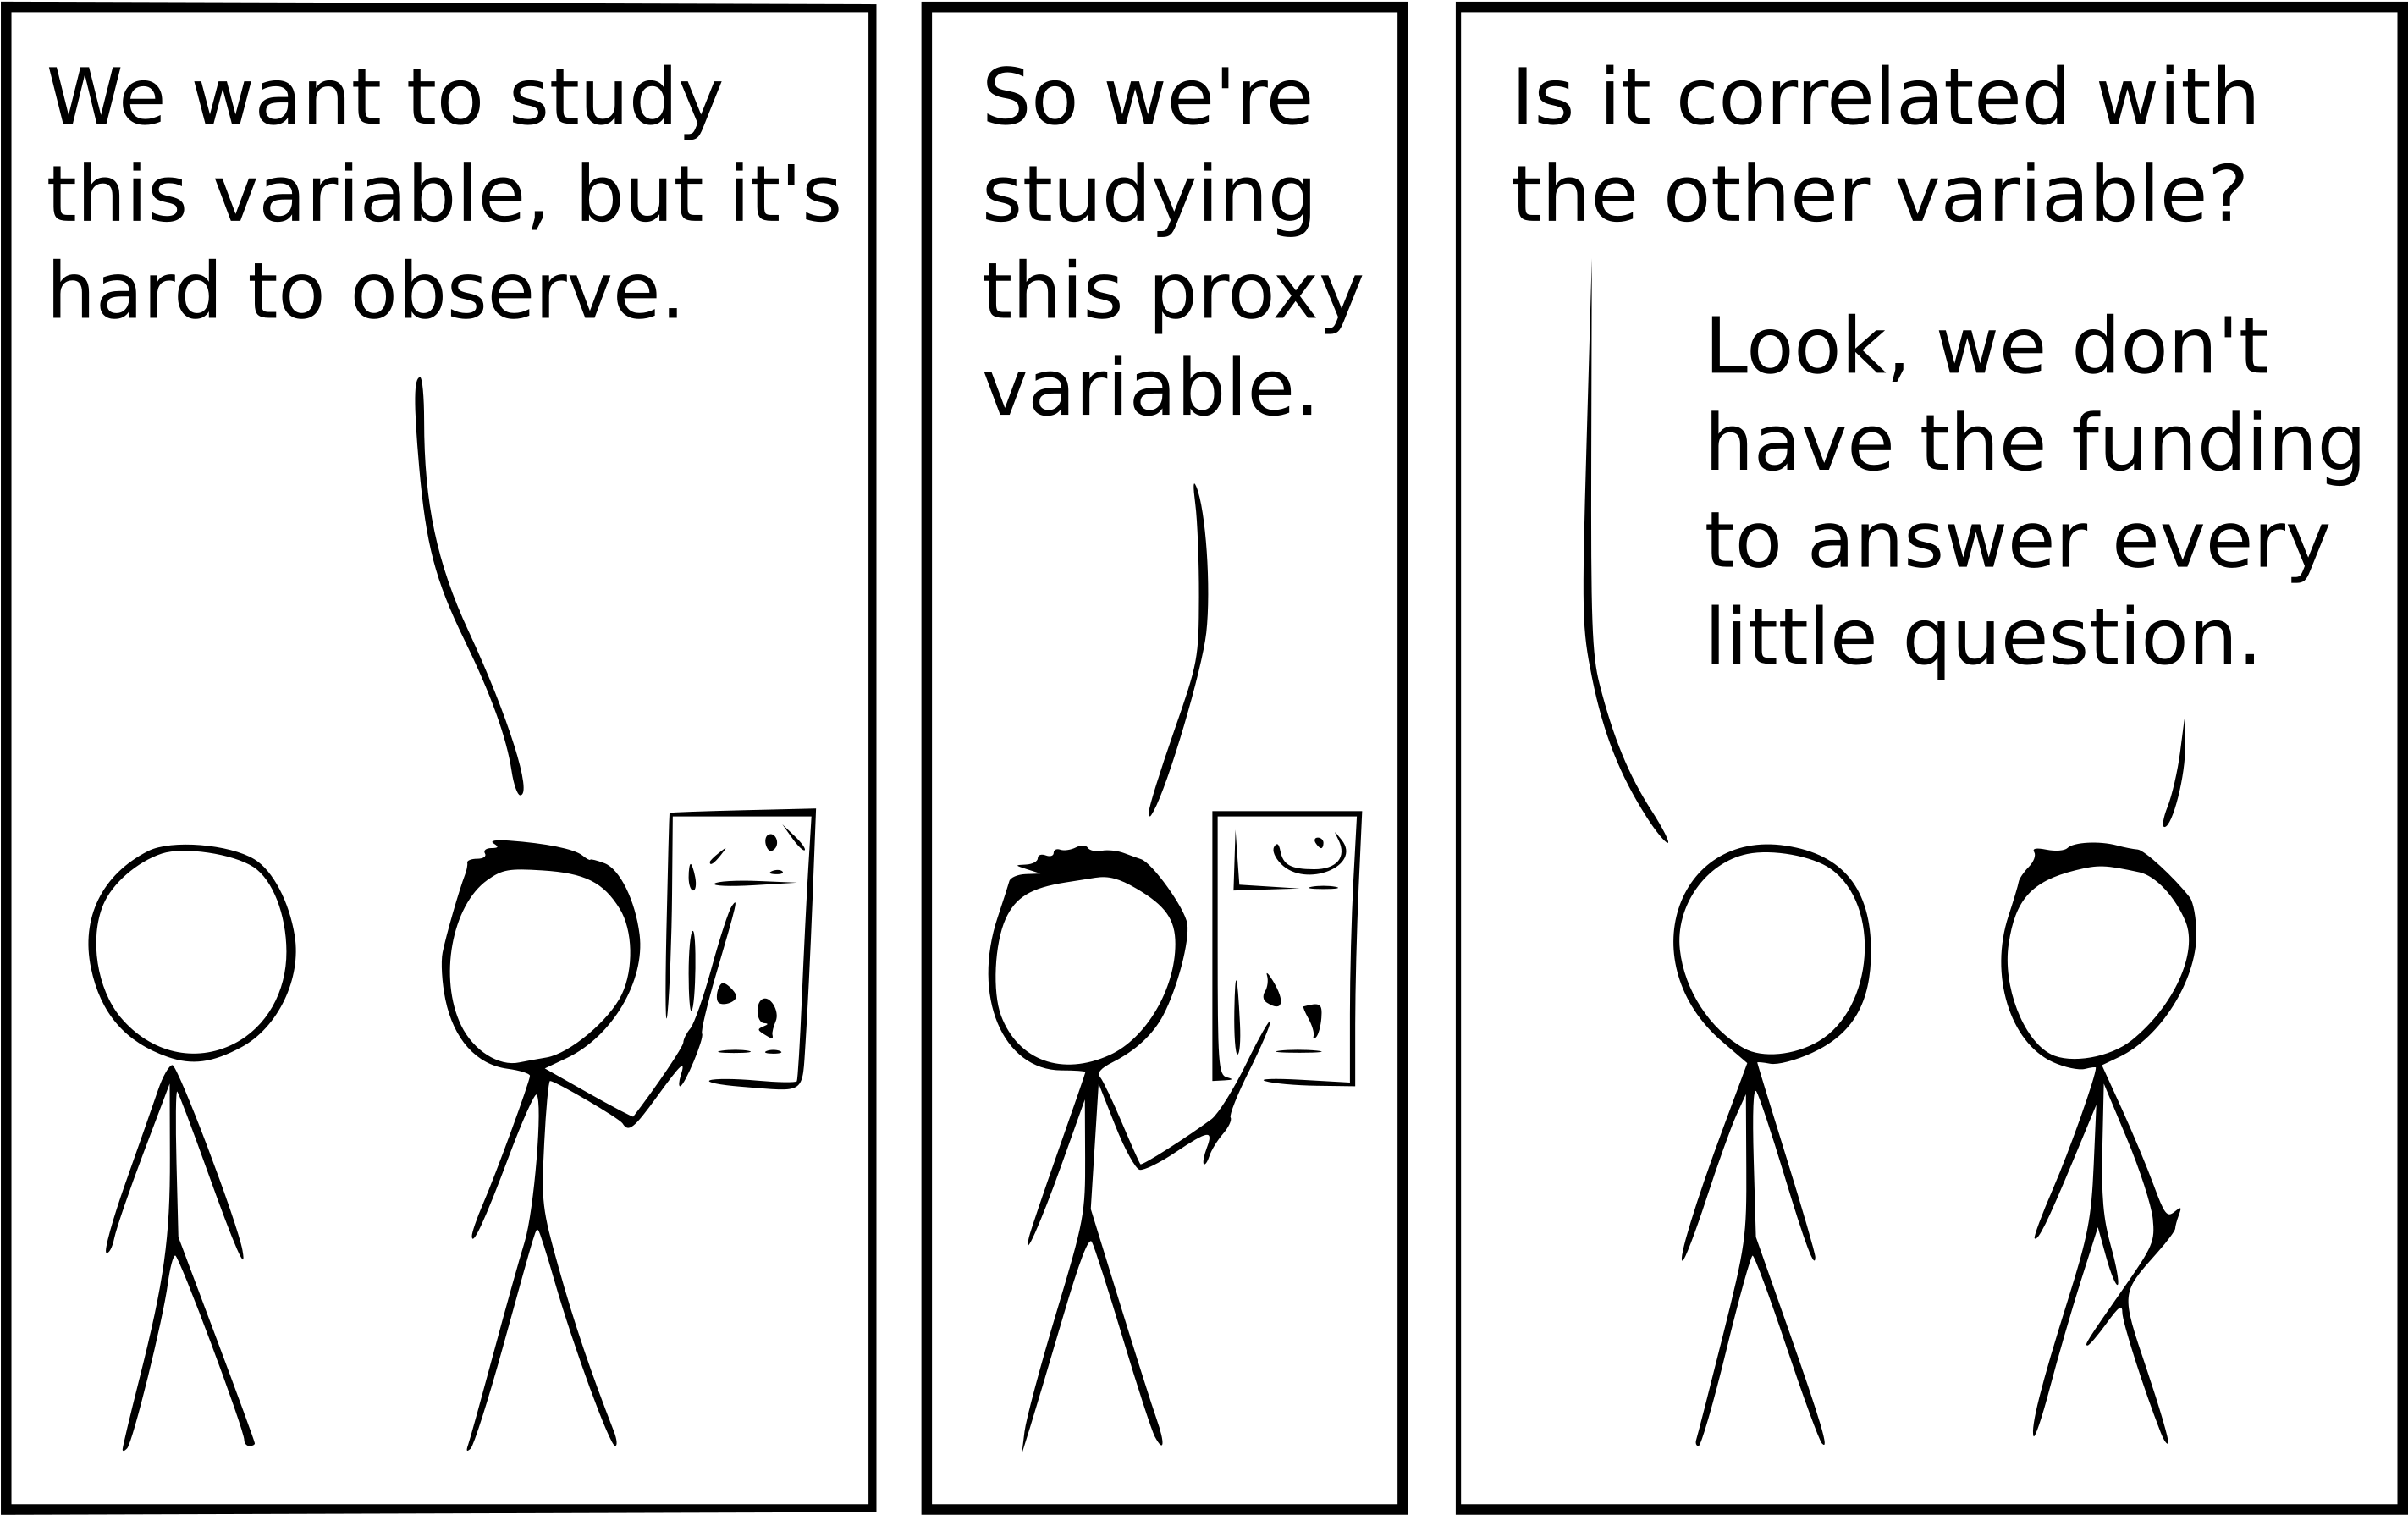
\includegraphics[width=\linewidth]{ch.discussion/imgs/xkcd_proxy.png}
    \caption{\textbf{RNA-seq is used as a proxy for gene regulation and protein expression}, but its relation to those is bad correlation TODO remains poorly understood. \textbf{xkcd}. URL: https://xkcd.com/2652}
    \label{fig:xkcd_proxy}
\end{figure}

\subsubsection{Universal gene regulatory networks}

In chapter X we discuss that single cell, multi-omics, and neural networks. Now I realize that a fourth final, is universal networks. It is kinda implicit in neural networks, as NNs often model multple cell states.

\begin{enumerate}
    \item Comparison between two cases can not make predictions
    \item more data to train
    \item in the end single set of instructions (DNA)
\end{enumerate}

It doesn't make sense to make GRNs between two specific cell types, or two developmental stages. There is a single set of instructions (DNA). So it should be possible to have a single universal GRN. (e.g. avocado).

Moreover, perhaps it is important to ask ourselves what is ultimately the goal of these GRNs? Do we care about having a map with all the arrows? Because the current correlation-based networks won't help us with differentiation networks. 

\section{Bioinformatics' technical debt}

Bioinformatics analyses are inherently complex due to the complicated nature of biology. This complexity is worsened by bioinformatics's dynamic and ever-evolving landscape, which continuously incorporates new technologies and insights. Adding to this complexity is the use of outdated, idiosyncratic, and poorly maintained software and file formats. This in turn leads bioinformaticians to more easily make mistakes and do duplicate work. In software development, this problem is known as "technical debt". Technical debt is analogous to financial debt, where you borrow money and must eventually pay it back, including interest. I am of the opinion that in the field of bioinformatics, the technical debt has become so large that it has become prohibitive for analyses.

The most common file formats in bioinformatics have been designed in the 90s and 00s, and as such reflect the tools of their time. Perl and awk were popular languages for bioinformatics, and for this reason, file formats are generally plain text and line-based. The sam, bam, bed, gtf, and vcf file formats all specify genomic features and their position, and are a great example of poorly thought-through design. The bam and bed format are zero-indexed\cite{Li2009}, whilst the sam-, gff, and vcf-format are one-indexed\cite{Li2009,Danecek2011}. This makes one-off errors between these formats extremely easy and incurs significant development time for anyone working with these files. An example of an outdated file format is the fasta file format which was developed in 1985\cite{Lipman1985}. Its age initially shows because lines are split over 80 characters, as that was the maximum screen width of the past. The true problem with the fasta format is, however, that it can not naturally represent uncertainty at genomic locations. Single nucleotide polymorphisms are represented by their IUPAC codes, but uncertainties longer than a single nucleotide can not be naturally represented. The solution for this problem is to append alternative sequences to the fasta. These sequences can then alternatively be used by for instance a genomic aligner. However, bwa mem(2)\cite{bwamem,bwamem2}, and Illumina Dragen are the only genomic aligners that support this, even though alternative regions are added to the human genome since 2013. More confusing is the slow adoption of updated genomes. Google Scholar reports 7,630 publications that make use of  hg19 or grch37 in 2023, whilst only 8,960 publications in 2023 make use of hg38 or grch38. The T2T-CHM13 assembly from 2022 only has 222 citations so far this year. Not surprisingly, a better genome assembly results in more accurate clinical discoveries \cite{Aganezov2022}.

A project with significant technical debt is the Sequencing Read Archive (SRA), which shares enormous amounts of public sequencing data. The SRA has been essential for my Ph.D. research, as I have relied solely on public data. For chapter scpepa (chapter \textbf{TODO}), we aimed to download all available human H3K27ac data (12,000 samples) from the SRA as a reference database. Processing these samples meant that we had to download 20TB from the SRA and spent approximately 300,000 CPU hours processing them on Cartesius, costing €1,000 for the SRA\cite{amazon}, €9,000 for Cartesius, and emitting nearly one tonne of CO2\cite{CO2}. In the analysis that followed, however, it turned out that obtaining sample annotations, such as tissue or cell type, is challenging due to the lack of standardized metadata on the SRA. Third-party tools like MetaSRA\cite{Bernstein2017}, and PredictMEE\cite{Klie2021} have been developed to automatically infer this metadata but did not resolve my issues. In the end, we decided to discard the experiment. 

Not only is the SRA missing crucial metadata, but the sra-tools, a toolkit for downloading sequencing data, are also particularly difficult to use. As a consequence, many alternative tools have been developed for downloading data from the SRA, such as the SRA-explorer\cite{sraexplorer}, pysradb\cite{pysradb}, FetchFastQ\cite{galvez2022metadata}, nf-core/fetchngs\cite{fetchngs}, the seq2science download-fastq workflow\cite{seq2science}, and parallel-fastq-dump\cite{parallelfastq}. Similarly, the submission of new sequencing data is notoriously complicated, causing people to make mistakes, which even leads to others developing tools to streamline this process\cite{Quiones2020}. During my Ph.D., I have come across many instances of data being mislabeled or missing presumably because of the difficult upload process.

One of the most popular tools in bioinformatics is the peak caller MACS(2), which has been cited more than 14,000 times\cite{Zhang2008}. MACS2 has been continuously developed since 2008, and its developers should get credit for this effort. Nevertheless, MACS2 is a particularly poorly designed software tool, and especially idiosyncratic with ATAC-seq peak-calling. The recommended way to use MACS2 in the case of ATAC-seq discards all mates from paired-end data. A similarly surprising design choice is that MACS2 did not support more than two replicates (until I implemented it). Genrich, a practically identical peak caller has been developed by another group as an alternative to MACS2\cite{Gaspar2018}.

\begin{figure}[H]
    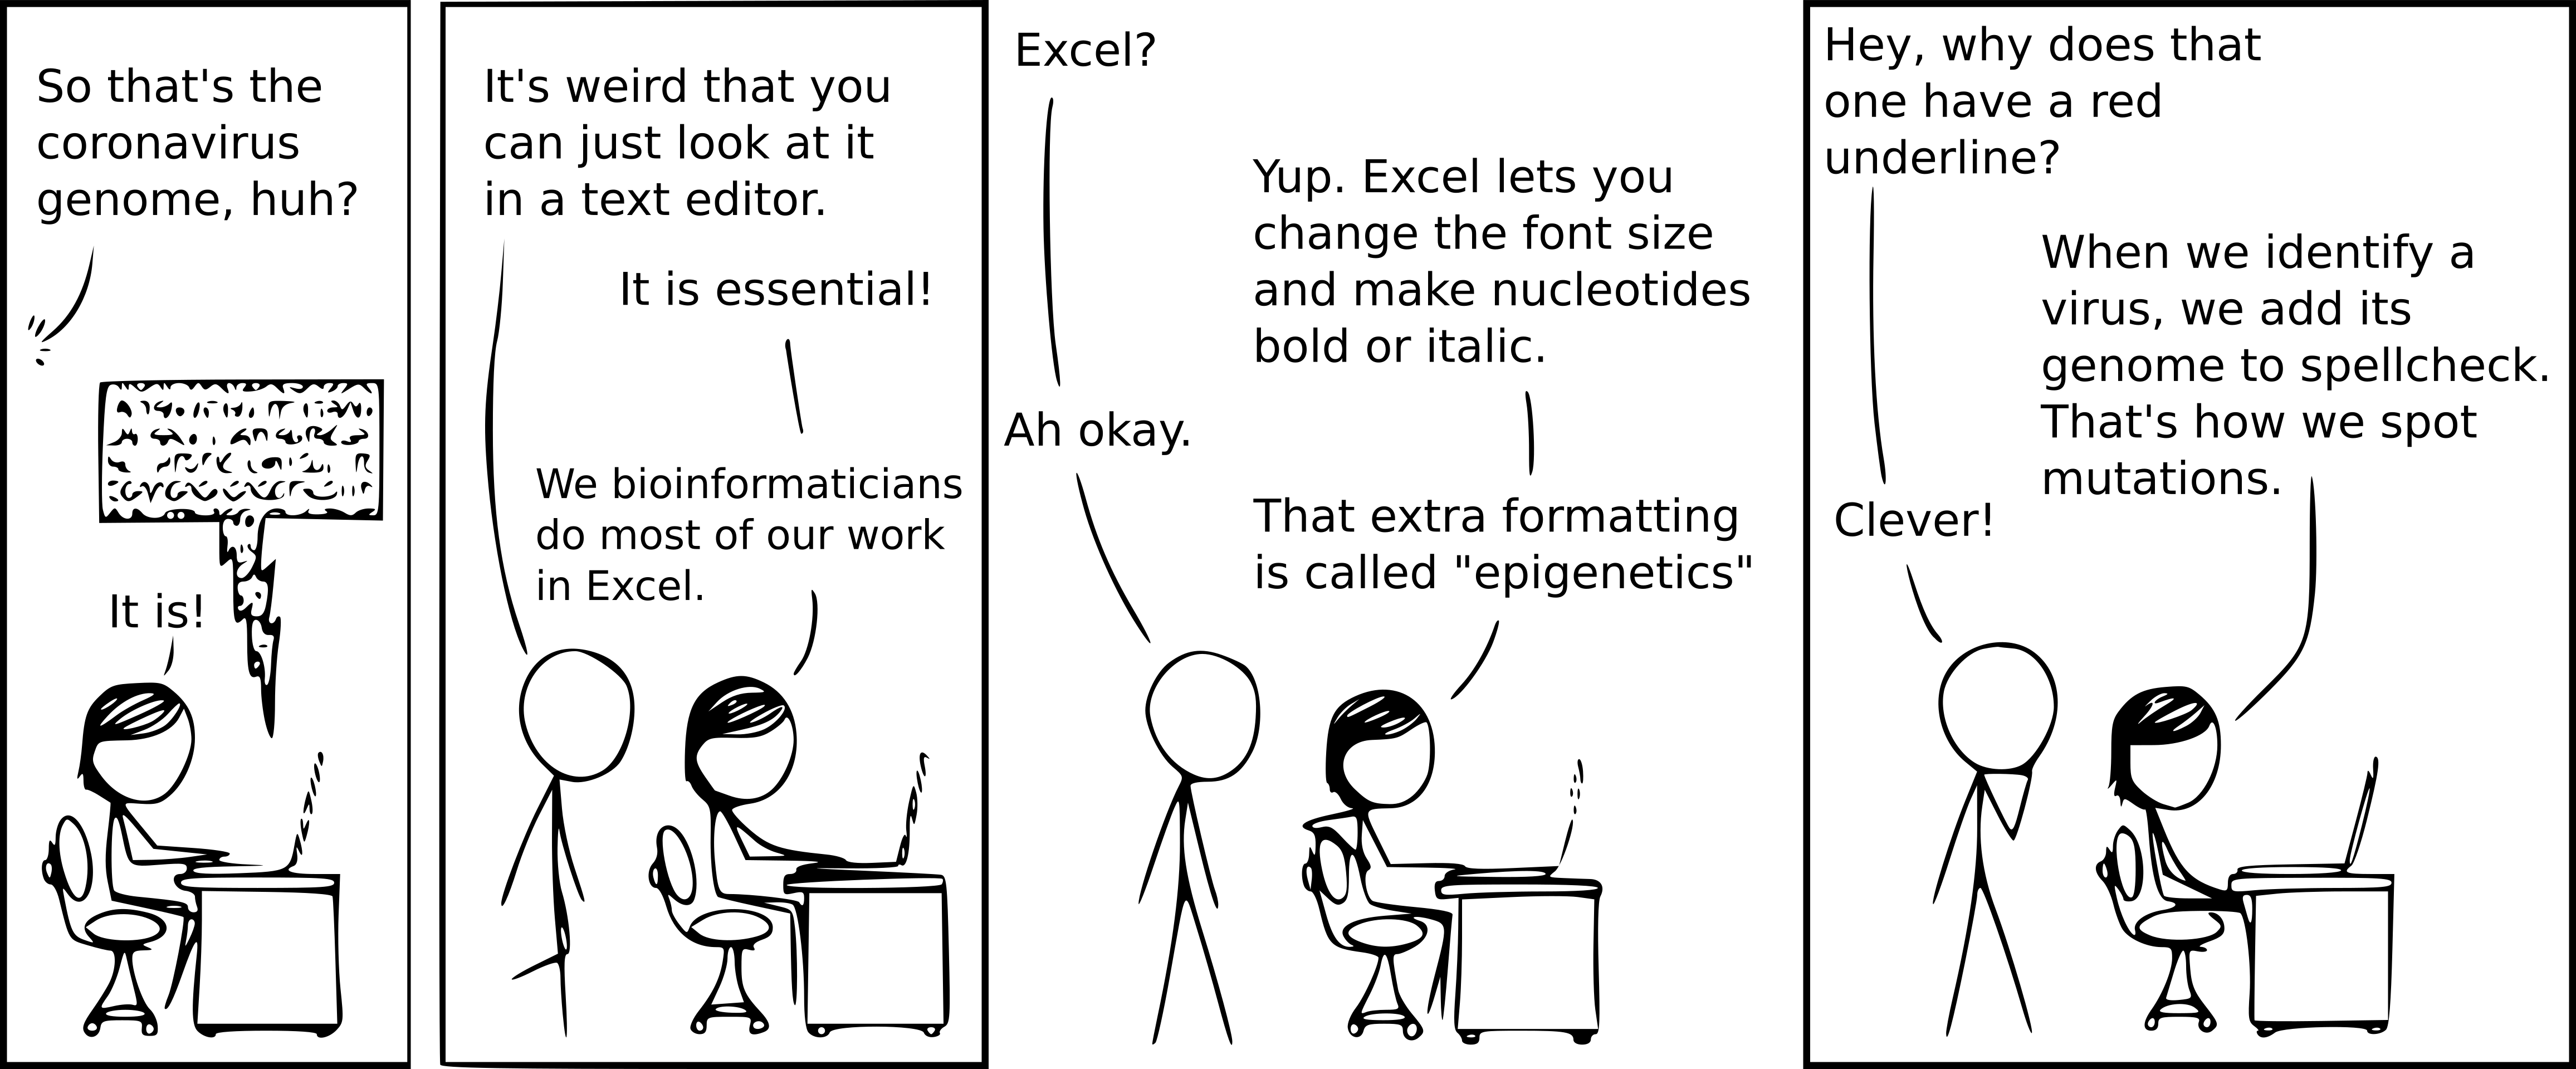
\includegraphics[width=\linewidth]{ch.discussion/imgs/xkcd_excel.png}
    \caption{\textbf{The use of Excel is surprisingly common in bioinformatics.} The popularity of Excel can be attributed to the lack of (formal) training of bioinformaticians, as it is a particularly bad tool for the job. Excel notoriously mangles gene names\cite{Zeeberg2004} and is a bad database format. For example, the gene SEPT1 gets converted into September 1, and approximately $30\%$ of studies report mangled gene names\cite{Abeysooriya2021}. Similarly, the use of Excel as a database is wholly inappropriate. For example, the UK government used the XLS (Excel file format) to store COVID test results. But as the XLS format is limited to 65,000 rows of data, the test results of the 65,001\textsuperscript{st} test and later were lost\cite{bbc_excel}.
    \textbf{xkcd}. URL: https://xkcd.com/2298/}
    \label{fig:xkcd_excel}
\end{figure}

Finally, the quickest developing part of molecular analyses currently is the field of single-cell analyses. As a consequence, the most technical debt is taken in these parts. Single-cell tools are usually implemented poorly, taking days to run and requiring enormous amounts of memory. The usual solution to this problem is not to improve the implementation, but instead to increase the hardware capacity. For instance, an ex-colleague requested 4TB of RAM for his computer at his new position. A particularly painful point of technical debt is the implementation of the log fold change calculation of Seurat. Seurat calculates the log of the means (as opposed to the mean of the logs), which makes it sensitive to outliers and should be changed. This results in vastly different outcomes depending on whether one used Seurat or an alternative tool such as Scanpy for their analysis. The bug was reported in November 2022, got an incomplete fix in March 2023, and as yet has not been fixed (https://github.com/satijalab/seurat/issues/6654). Seurat has been cited 7,699 times\cite{Butler2018}.

Taking \textit{deliberate} technical debt is okay. Sometimes you just have to develop fast, and often it is not even clear if something will work out. The problem with bioinformatics is, however, that a large part of the technical debt is taken inadvertently. I think the two main reasons for this are the lack of bioinformatics training, and the lack of interdepartmental collaborations on software. Two things, in hindsight, that were also missing during my Ph.D. 

Because the field of bioinformatics is so young and rapidly becoming more important the supply of bioinformaticians is lacking behind their demand. This in turn leads to biologists starting bioinformatics analyses without formal training. This is a widely accepted fact in the field, and even facilitated by projects such as Galaxy\cite{galaxy}. In turn, bioinformaticians without formal training in programming, statistics, or modeling are  developing tools and file formats, and doing analyses, which simply means their quality and correctness are low. Without exception, every time I thoroughly delved into the methodology of analyses I found major issues, for example, chapters \textbf{X} and \textbf{Y} or PUBPEER?. It is surprising that the idea prevails that anyone should be able to do a bioinformatics analysis, while wet lab work is typically restricted to those who have undergone formal training. If we continue to fail to train the next generation of biologists in bioinformatics, we risk hindering progress in the field.

Another part of the problem is that most tools are developed independently, most of the time by a single Ph.D. student or postdoc. This has two major downsides. The first is that the maintenance of tools depends on individuals. If someone decides to leave academia, their tools, how useful they might be, will soon become obsolete as no one will maintain them. Second, most tools are unnecessarily specialized for the task the developer is trying to solve. This in turn leads to many near-identical implementations that solve the same problem, e.g. fastq downloading. These problems should be overcome if bioinformaticians would develop more in collaborations. A collaboration between multiple groups and multiple expertise levels would make sure projects are not abandoned when a person leaves and would make sure that tools are useful for wider groups. 

In conclusion, while the field of bioinformatics has enabled significant scientific discoveries, it grapples with a substantial and growing technical debt. Addressing these issues requires collaboration, improved training, and a shift toward more sustainable and efficient practices. Failure to do so will hinder future advancements.
